\begin{frame}
	\frametitle{Latest application of \chemfig{B_2 pin_2}\footfullcite{RN9}}
	\begin{figure}
		\centering
		\includegraphics[width=0.8\linewidth]{fig/b2pin2-intro}
		\label{fig:b2pin2-intro}
	\end{figure}
	
\end{frame}

\begin{frame}
	\frametitle{Synthetic Applications of the New Method}
	When applied with \chemfig{B_2 pin_2}, p-PhPy, MeOK, the following reactions can take place\footfullcite{Pyridine}:
	\begin{figure}
		\centering
		\includegraphics[width=0.44\linewidth]{fig/b2pin2-showcase}
		\label{fig:b2pin2-showcase}
	\end{figure}
	
\end{frame}

\begin{frame}
	\frametitle{Mechanisms of this Method}
	\begin{figure}
		\centering
		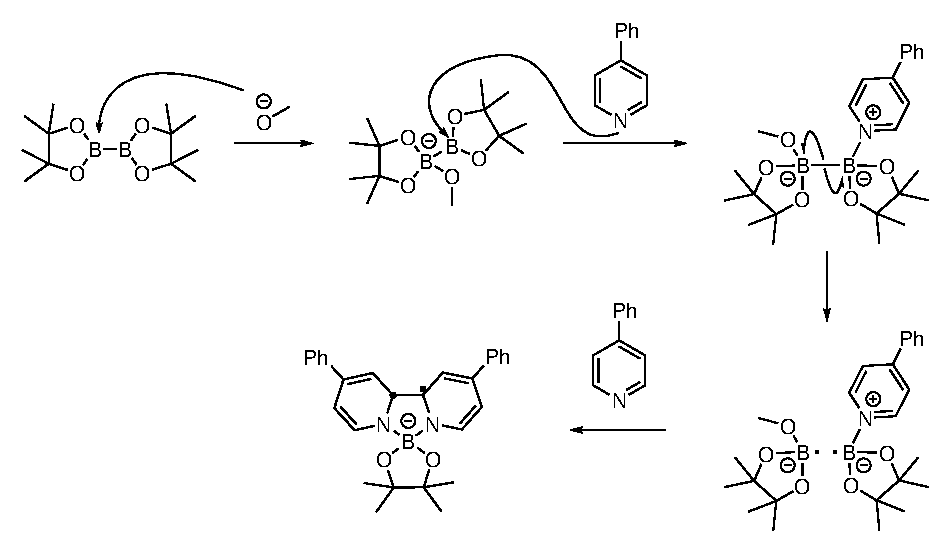
\includegraphics[width=0.8\linewidth]{fig/b2pin2mech}
		%\caption{}
		\label{fig:b2pin2mech}
	\end{figure}
	
\end{frame}